\documentclass[12pt, a4paper, oneside]{article}\usepackage[]{graphicx}\usepackage[]{color}
%% maxwidth is the original width if it is less than linewidth
%% otherwise use linewidth (to make sure the graphics do not exceed the margin)
\makeatletter
\def\maxwidth{ %
  \ifdim\Gin@nat@width>\linewidth
    \linewidth
  \else
    \Gin@nat@width
  \fi
}
\makeatother

\definecolor{fgcolor}{rgb}{0.345, 0.345, 0.345}
\newcommand{\hlnum}[1]{\textcolor[rgb]{0.686,0.059,0.569}{#1}}%
\newcommand{\hlstr}[1]{\textcolor[rgb]{0.192,0.494,0.8}{#1}}%
\newcommand{\hlcom}[1]{\textcolor[rgb]{0.678,0.584,0.686}{\textit{#1}}}%
\newcommand{\hlopt}[1]{\textcolor[rgb]{0,0,0}{#1}}%
\newcommand{\hlstd}[1]{\textcolor[rgb]{0.345,0.345,0.345}{#1}}%
\newcommand{\hlkwa}[1]{\textcolor[rgb]{0.161,0.373,0.58}{\textbf{#1}}}%
\newcommand{\hlkwb}[1]{\textcolor[rgb]{0.69,0.353,0.396}{#1}}%
\newcommand{\hlkwc}[1]{\textcolor[rgb]{0.333,0.667,0.333}{#1}}%
\newcommand{\hlkwd}[1]{\textcolor[rgb]{0.737,0.353,0.396}{\textbf{#1}}}%

\usepackage{framed}
\makeatletter
\newenvironment{kframe}{%
 \def\at@end@of@kframe{}%
 \ifinner\ifhmode%
  \def\at@end@of@kframe{\end{minipage}}%
  \begin{minipage}{\columnwidth}%
 \fi\fi%
 \def\FrameCommand##1{\hskip\@totalleftmargin \hskip-\fboxsep
 \colorbox{shadecolor}{##1}\hskip-\fboxsep
     % There is no \\@totalrightmargin, so:
     \hskip-\linewidth \hskip-\@totalleftmargin \hskip\columnwidth}%
 \MakeFramed {\advance\hsize-\width
   \@totalleftmargin\z@ \linewidth\hsize
   \@setminipage}}%
 {\par\unskip\endMakeFramed%
 \at@end@of@kframe}
\makeatother

\definecolor{shadecolor}{rgb}{.97, .97, .97}
\definecolor{messagecolor}{rgb}{0, 0, 0}
\definecolor{warningcolor}{rgb}{1, 0, 1}
\definecolor{errorcolor}{rgb}{1, 0, 0}
\newenvironment{knitrout}{}{} % an empty environment to be redefined in TeX

\usepackage{alltt} % Paper size, default font size and one-sided paper
%\graphicspath{{./Figures/}} % Specifies the directory where pictures are stored
%\usepackage[dcucite]{harvard}
\usepackage{rotating}
\usepackage{setspace}
\usepackage{pdflscape}
\usepackage[flushleft]{threeparttable}
\usepackage{multirow}
\usepackage{amsmath}
\usepackage[comma, sort&compress]{natbib}% Use the natbib reference package - read up on this to edit the reference style; if you want text (e.g. Smith et al., 2012) for the in-text references (instead of numbers), remove 'numbers' 
\usepackage{graphicx}
%\bibliographystyle{plainnat}
\bibliographystyle{agsm}
\usepackage[colorlinks = true, citecolor = blue, linkcolor = blue]{hyperref}
%\hypersetup{urlcolor=blue, colorlinks=true} % Colors hyperlinks in blue - change to black if annoying
%\renewcommand[\harvardurl]{URL: \url}
\IfFileExists{upquote.sty}{\usepackage{upquote}}{}
\begin{document}
\title{Questions on Calculus}
\author{Rob Hayward} 
\date{\today}
\maketitle

\doublespacing
\begin{enumerate}


\item What are the drivatives of
\begin{itemize}
\item $y = 2 + 6x$

$\frac{d(y)}{d(x)} = $

\item $y = 5 - 4x +2x^3$

$\frac{d(y)}{d(x)} = $

\item $y = 25 +6x^2 - 3x^3 +25x^4$

$\frac{d(y)}{d(x)} = $

\item $y - 3 = 2x$

$\frac{d(y)}{d(x)} = $

\item $TPP = 24 +5L +2L^2 - L^3$

$\frac{d(TPP)}{d(L)} = $

Find the second derivative of the following

\item $TU = 25 + X_1 - X_1^2$

$\frac{d^2(U)}{d(X_1)^2} = $

\item $TU = 25 +25X_1 -2X_1^2$

$\frac{d^2(U)}{d(X_1)^2} = $

\item $TPP = 15 +15Q +Q^2 - Q^3$

$\frac{d^2(TPP)}{d(L)^2} = $

\item What does your answer to the previous question tell you about the shape of the Total Physical Product Curve? 


\item Given the $TU = 25X - 0.5X^2$
\begin{itemize}
\item What is the drivative of TU?

$\frac{d(TU)}{{dX}} = $

\item What can we say about the utility of X?



\end{itemize}

Given a demand curve 
\begin{equation*}
Q_d = 90 - 5P + 0.2P^2
\end{equation*}

\begin{knitrout}
\definecolor{shadecolor}{rgb}{0.969, 0.969, 0.969}\color{fgcolor}
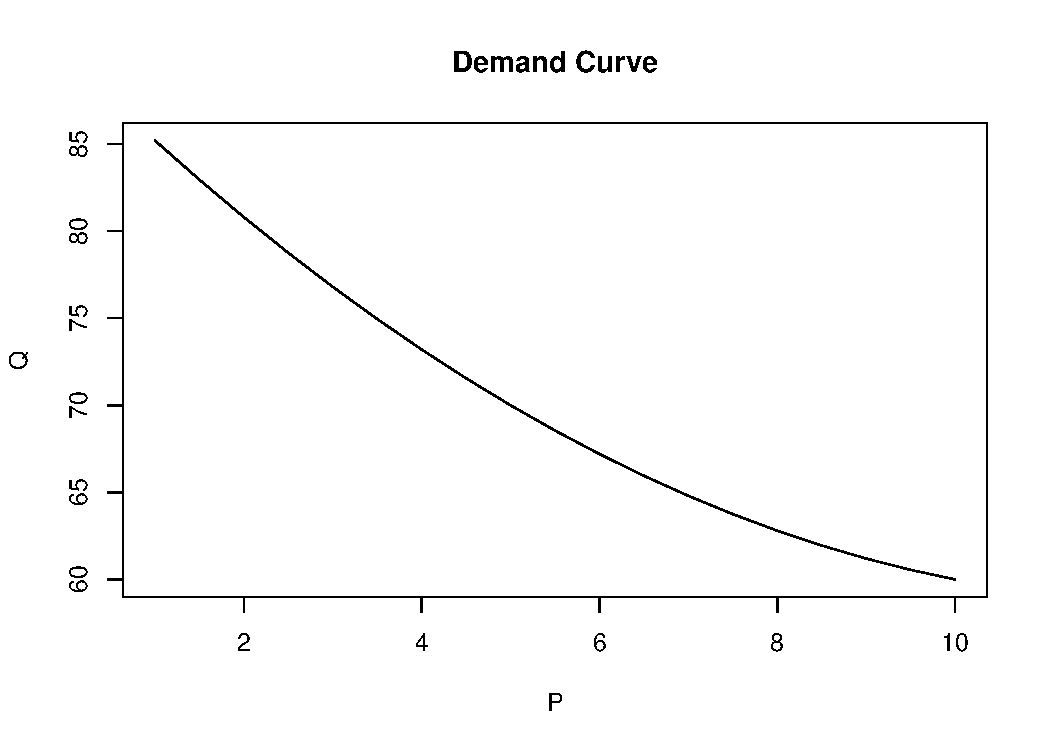
\includegraphics[width=\maxwidth]{figure/plot3-1} 

\end{knitrout}

What is the elasticity of demand at the point $P = 5, Q = 70$?  



\item Here is the total physical product curve. Draw the \emph{average physical product}? for between two points on the graph. 

  
\begin{knitrout}
\definecolor{shadecolor}{rgb}{0.969, 0.969, 0.969}\color{fgcolor}

{\centering 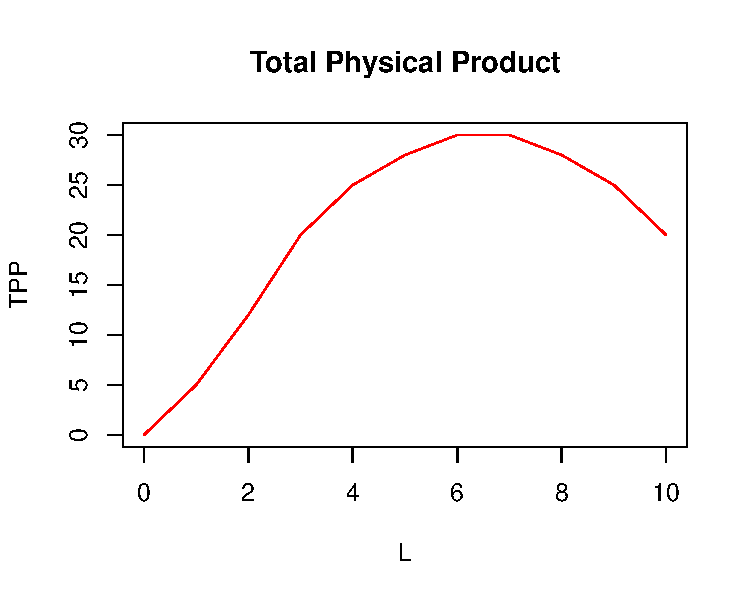
\includegraphics[width=\maxwidth]{figure/plot-1} 

}



\end{knitrout}
\item How would you calculate the \emph{marginal physical product}?

\end{itemize}

\item What is the gradient of the TPP at its peak? 

\item What is the value of the MPP when TPP is at its peak? 

\item Given the $TPP = 100 + 32Q +23Q^2 - Q^3$, 
\begin{itemize}
\item What is the TPP' or MPP?

\item How would you find the maximum TPP? What is the maximum TPP? This can be done with factorisation. 

\end{itemize}

\item Given the $TPP = 500 + 180Q + 15Q^2 - 2Q^3$, 
\begin{itemize}
\item What is the TPP' or MPP?

$MPP = 180 + 30Q -6Q^2$

\item What is the maximum TPP? The equaition.

\end{itemize}


\end{enumerate}
\end{document}
